\section{Simulation Results} \label{opsimresult}

To validate that the calculations have been made correctly, an open loop simulation of the circuit was conducted. As it can be seen in figure \ref{fig:openloop_schematic} the circuit consists of the 4 MOSFETs, the inductor, the 2 capacitors and a load. The MOSFETs are controlled with two duty cycles D1 and D2. FET1 and FET4 will get the actual duty cycle while FET2 and FET3 uses the inverted duty cycles. With the scope the output voltage and current through the inductor can be visualized.

\begin{figure}[H]
	\begin{center}
		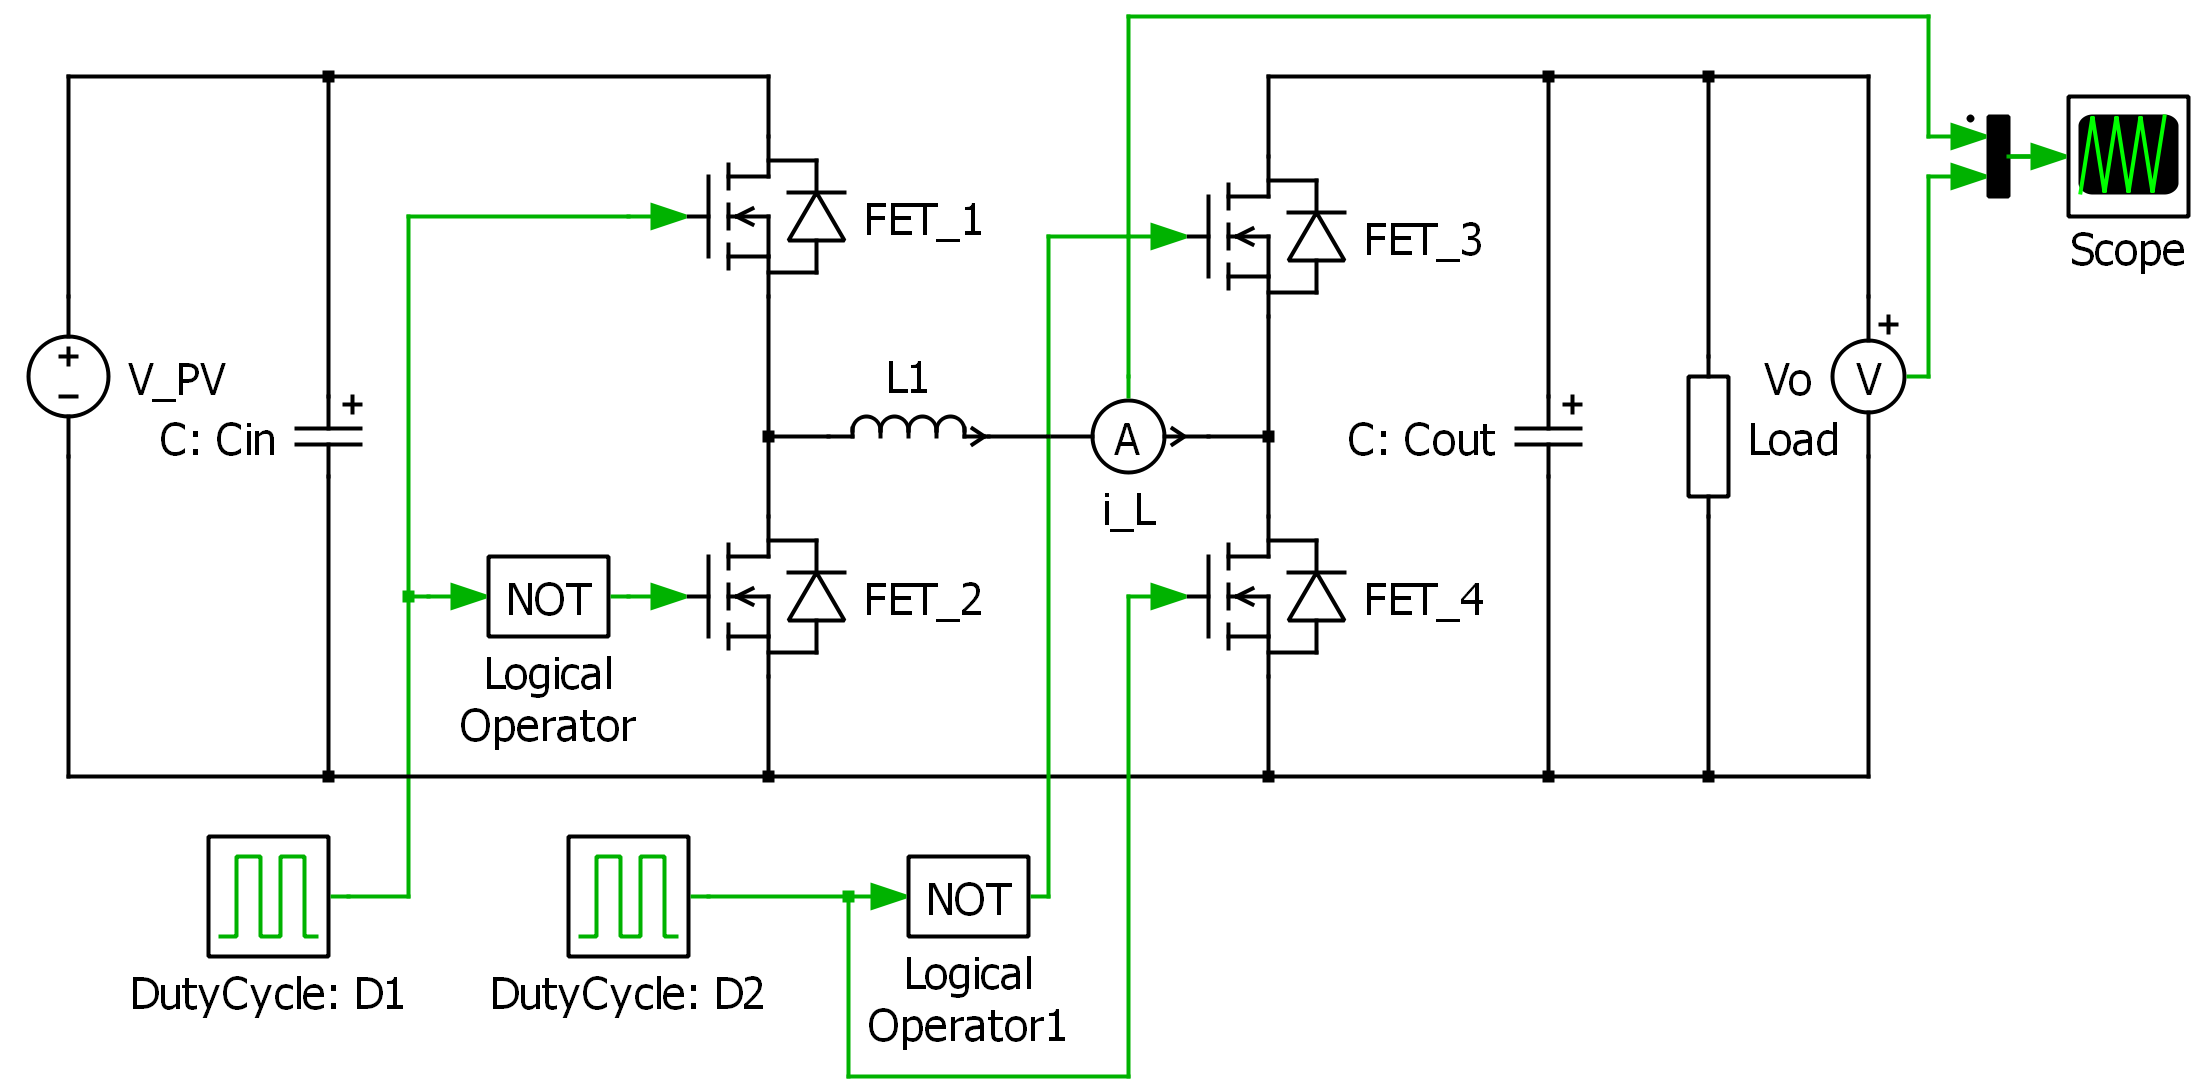
\includegraphics[width=0.8\textwidth]{../Pictures/P1/Open_loop_simulation/open_loop_schematic}
		\caption{Ideal open-loop simulation.}
		\label{fig:openloop_schematic}
	\end{center}
\end{figure}
The values for the components are $C_{in}=1.54mF$, $C_{out}=88 \mu F$ and $L1=1.3mH$ as calculated in section \ref{component_sizing}. At first the buck mode is simulated. In this mode D2 is 0. This means that FET4 is off and FET3 is on. To achieve the minimum output voltage at $24V$, the corresponding duty cycle is calculated in equation \ref{eq:ol_duty_buck}. The load resistor is calculated for maximum output power for the PV-panel in equation \ref{eq:ol_load_buck}.
\begin{equation} \label{eq:ol_duty_buck}
	D= \frac{V_{out}}{V_{in}} = \frac{24V}{36.9V} = 0.65
\end{equation}

\begin{equation} \label{eq:ol_load_buck}
	R_{load} = \frac{V^2}{P_{max}} = \frac{24V^2}{300W} = 1.92 \Omega
\end{equation}



\begin{figure}[H]
 	\begin{center}
 		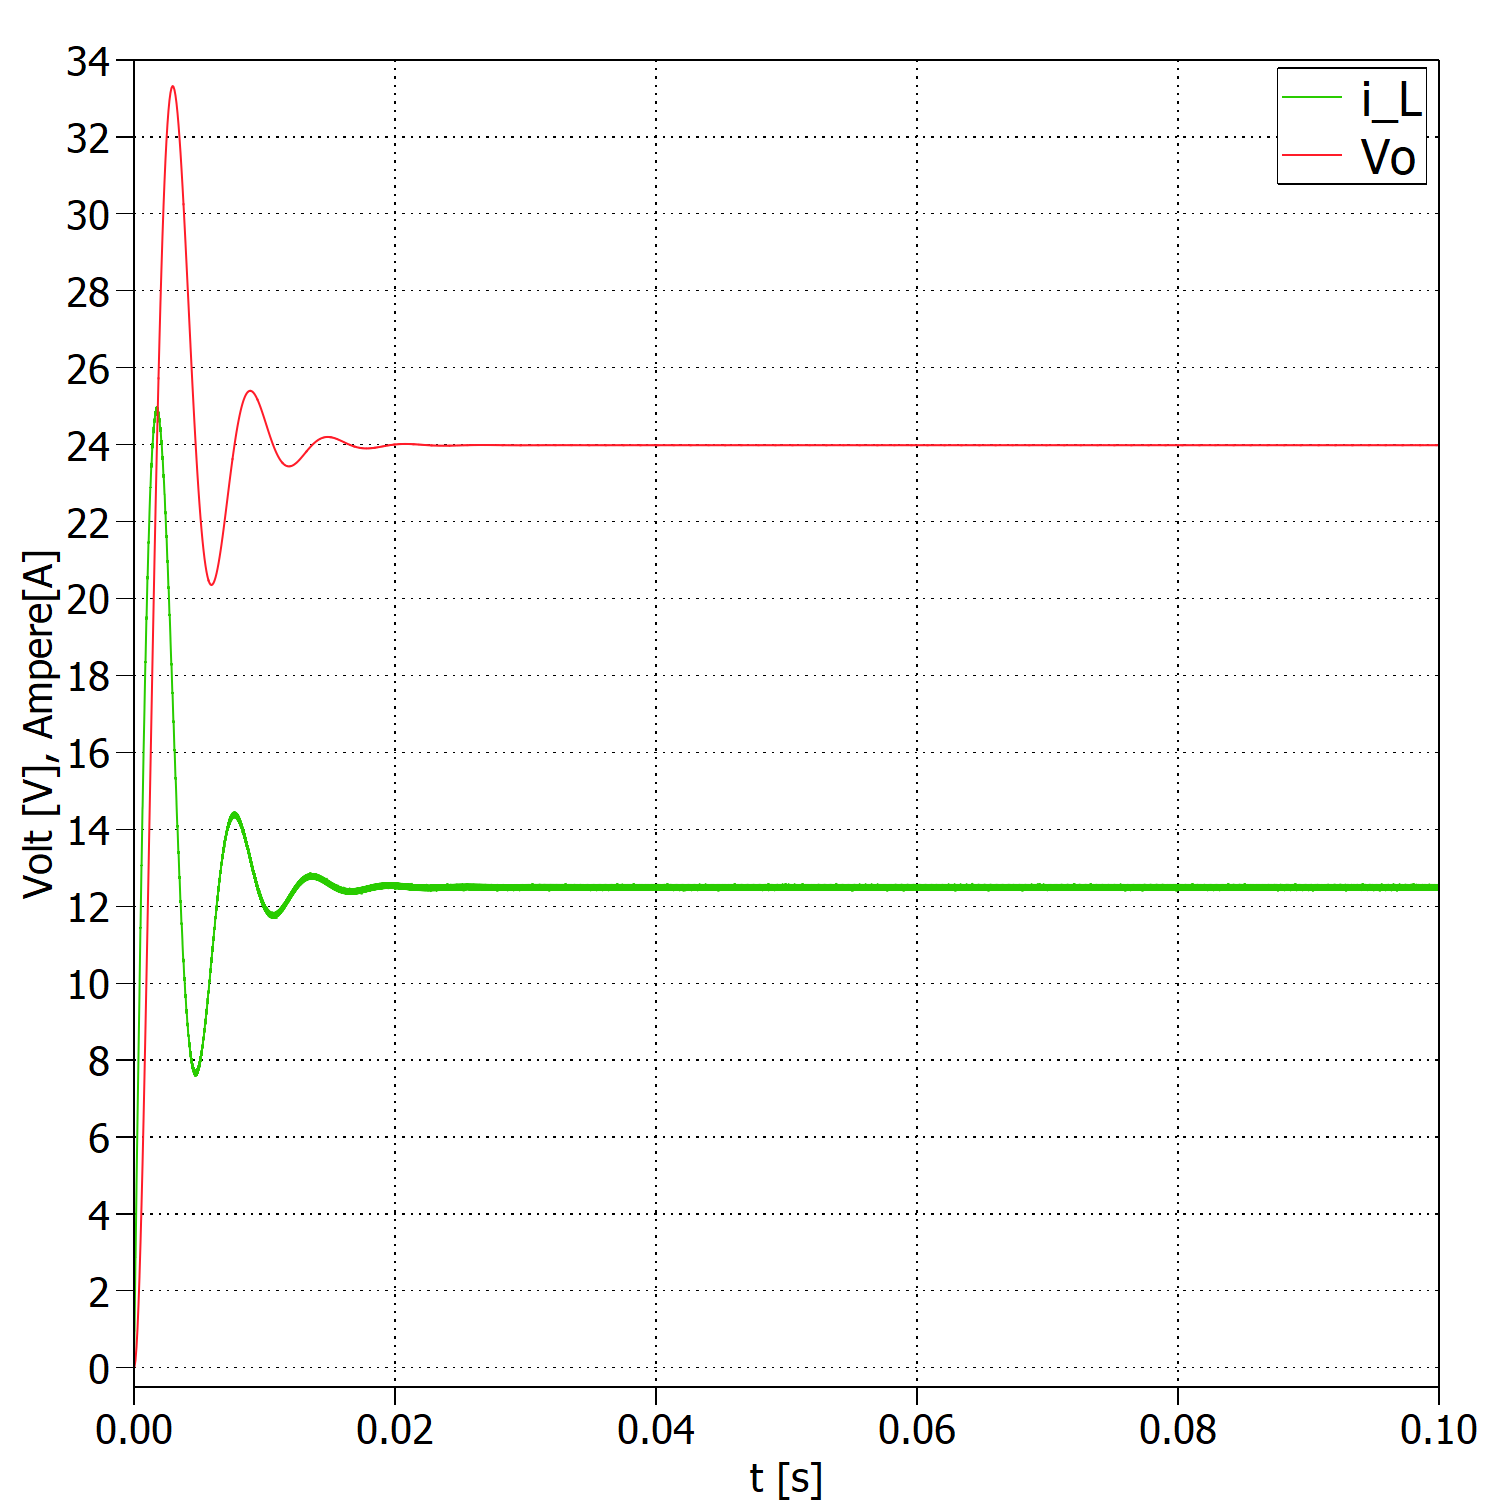
\includegraphics[width=0.6\textwidth]{../Pictures/P1/Open_loop_simulation/open_loop_buck}
 		\caption{Open-loop simulation in buck mode.}
 		\label{bucksimulation}
 	\end{center}
\end{figure} 
\todo{Fix this figure. The linewidth of the signals isn't the same and the axis names are small. Stef }

In buck mode the current through the inductor should be equal to the output current \ref{iavg} \todo{which ref is this? Stef} which with a load of $1.92\Omega$ should be:
\begin{equation}
I_{out} = \frac{V_{out}}{R_{load}} = \frac{24V}{1.92\Omega} = 12.5A
\end{equation}   

To simulate the boost mode the input voltage is the same. Here the duty cycle for D2 is 0.638. This should correspond to an output voltage of 90V and calculated with the same equation as \ref{boostD} \todo{Check!}. D1 is fixed to 1 so that FET1 is on and FET2 is off. This should give an output voltage of 90V. With 90V the output current should be 9A and then the current through the inductor is calculated like this:

\begin{equation}
I_{L} = \frac{1}{1-0.638}\cdot 12.5A = 9.207A
\end{equation}  
\todo{Equations should be first written with letters and after that put the values. Stef}

In figure \ref{boostsim} the red line is again the output voltage which is the expected 90V and the green line is the current through the inductor is a bit more than 9A \todo{a bit more? Be more precise. Stef}.

\begin{figure}[H]
	\begin{center}
		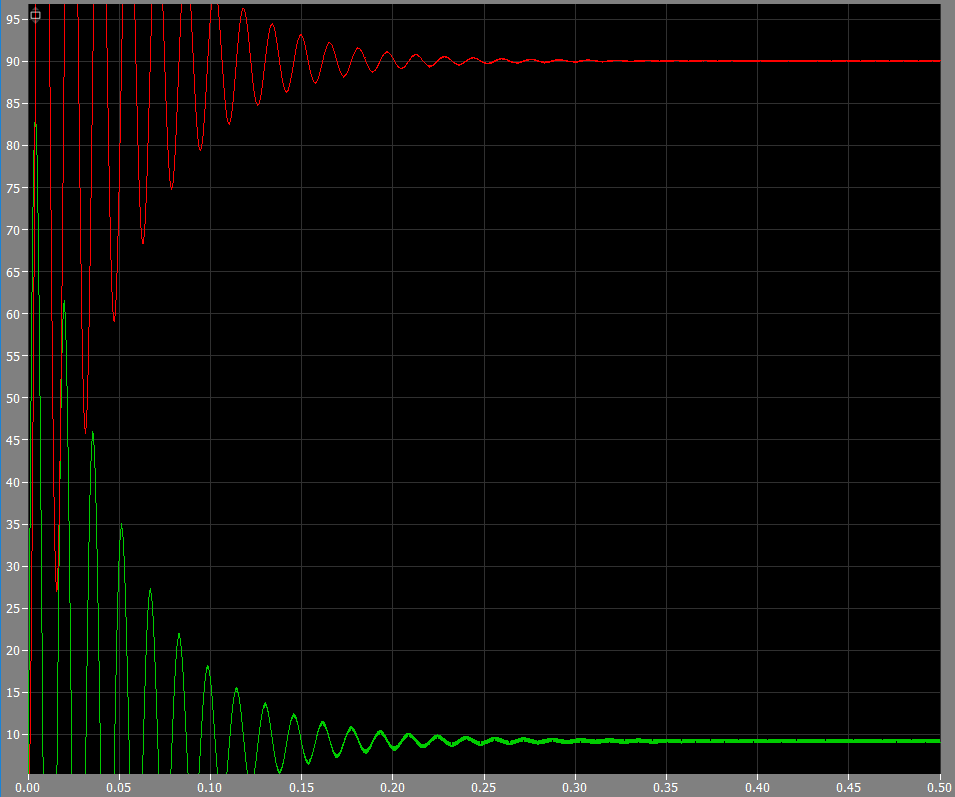
\includegraphics[width=0.5\textwidth]{../Pictures/boostsim}
		\caption{Open-loop simulation in boost mode.}
		\label{boostsim}
	\end{center}
\end{figure}

\todo{This figure will be updated.}